\chapter{Social connectedness index II from Facebook}

\resp{Lorenzo Vigorelli}

\section{Social Connectedness Index}
The Social Connectedness Index (SCI) measures the intensity of social ties between two locations $i$ and $j$ based on Facebook friendship links \cite{facebookSCI}. It is defined as

\begin{equation}
    SCI_{i,j} = \frac{FB\_Connections_{i,j}}{FB\_Users_i \cdot FB\_Users_j},
\end{equation}\\
where $FB\_Connections_{i,j}$ is the number of links between users in $i$ and $j$, and $FB\_Users_i$, $FB\_Users_j$ are the number of users in each location.  
The index expresses the relative probability of a friendship between $i$ and $j$, and is rescaled between $1$ and $1{,}000{,}000{,}000$ for comparability.  \\
To ensure data quality and privacy, locations with very few users are excluded, Gaussian noise is added to connection counts, values are averaged over multiple runs (covering approximately $99\%$ of users), and some regions are not reported.  
The resulting structure is an undirected, weighted graph where nodes correspond to geographic areas and edge weights to $SCI_{i,j}$.

\section{Dataset}
The dataset employed is the \texttt{GADM1NUTS3} snapshot of 15 December 2021, available through the Humanitarian Data Exchange portal \cite{gadm1nuts3countiescsv}.  
Geographic units are defined as follows:  
\begin{itemize}
    \item \textbf{Europe}: subdivided into NUTS3 regions according to Eurostat boundaries \cite{eurostatNUTS}.  
    \item \textbf{Canada and South Asia} (Bangladesh, India, Nepal, Pakistan, Sri Lanka): subdivided into GADM2 units; in the United States, counties are used following U.S. Census Bureau shapefiles \cite{uscensusCounties}.  
    \item \textbf{Other countries}: subdivided into GADM1 units, except those with a population below 1 million, which remain unsplit.  
\end{itemize}

Each row of the SCI file represents a pair of these regions. Geographic boundaries are sourced from the Database of Global Administrative Areas (GADM, versions 2.8 and 4.1) \cite{gadm}, with additional reference mapping files provided by Meta \cite{gadm1nuts2csv}.  

Since both the SCI collection methods and geographic codings have evolved over time, harmonization was required to align administrative levels.  
The ultimate objective is the construction, for each country, of an undirected weighted graph consisting of:  
\begin{itemize}
    \item a \textbf{node list}, including latitude and longitude (representative points of the regions);  
    \item an \textbf{edge list}, where edge weights correspond to the SCI values between regions.  
\end{itemize}

\section{Node list and edge list}

\textbf{Node list.}  
The set of nodes is obtained by intersecting the location codes in the SCI file (\texttt{user\_loc} and \texttt{fr\_loc}) with the reference table of admissible units \cite{gadm1nuts2csv}. The target granularities are \texttt{NUTS3}, \texttt{GADM2}, \texttt{GADM1}, and \texttt{COUNTY}. For each type, the corresponding geometries are loaded from GADM \cite{gadm}, Eurostat \cite{eurostatNUTS}, or U.S.\ Census Bureau shapefiles \cite{uscensusCounties}, converted to WGS84, and assigned a representative point to determine latitude and longitude.  
As the coding systems differ, keys are normalized before spatial matching (e.g.\ GADM2 $\rightarrow$ \texttt{ISO3.ADM1.ADM2\_1}, GADM1 $\rightarrow$ \texttt{ISO3.ADM1\_1}, U.S.\ counties $\rightarrow$ 5-digit \texttt{GEOID}). \\
To avoid duplicates, the following priority is adopted: all \texttt{NUTS3} and \texttt{COUNTY} units are retained, \texttt{GADM2} units are kept, and any \texttt{GADM1} unit already covered at GADM2 level is discarded.  
The final node list contains: \texttt{nodeID}, \texttt{nodeLabel}, \texttt{nodeName} (if available), \texttt{latitude}, \texttt{longitude}, and the dataset of origin.  \\
\textbf{Edge list.}  
From the SCI file, only pairs with both endpoints successfully mapped are retained. Self-loops are removed and the network is treated as undirected: duplicate pairs $(i,j)$ and $(j,i)$ are merged by averaging the \texttt{scaled\_sci} values. Edge weights correspond to the scaled SCI, and no thresholding is applied at this stage. Intra-country subnetworks are obtained by restricting edges to nodes within the same country.\\  
\textbf{Limitations.}  
The intended GADM v2.8 could not be used; instead, v3.x and later versions were adopted \cite{gadm}, which employ different identifiers and coverage. Consequently, some GADM2 units could not be matched, reducing coverage in countries where ADM2 is the main resolution. Additional challenges include heterogeneous code formats, representative points for multipolygons, and the SCI’s built-in privacy noise and minimum-user thresholds, which produce many very small edge weights.

\section{Network analysis}
As the SCI subnetworks for each country are complete and undirected, weighted versions of classical metrics are considered. Other analyses on the global network in appendix \ref{app:SCI}\\
\begin{figure}[h!]
    \centering
    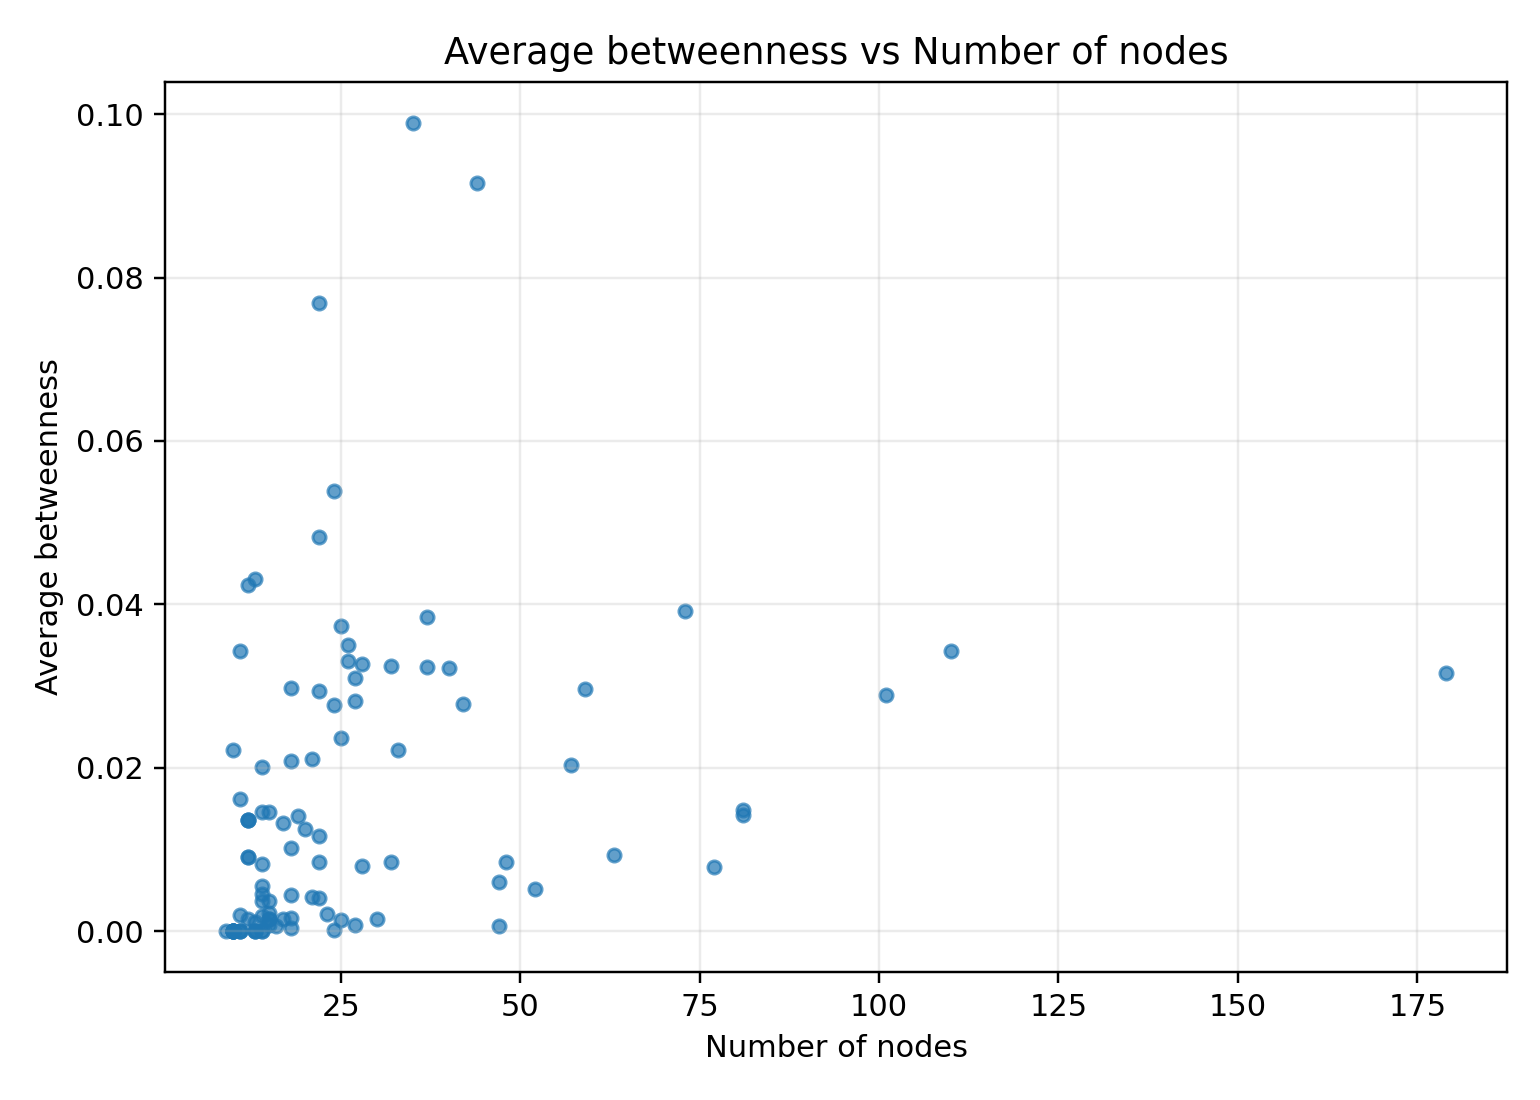
\includegraphics[width=0.45\textwidth]{images/TASK3/metrics_betweenness_avg_vs_n_nodes.png}
    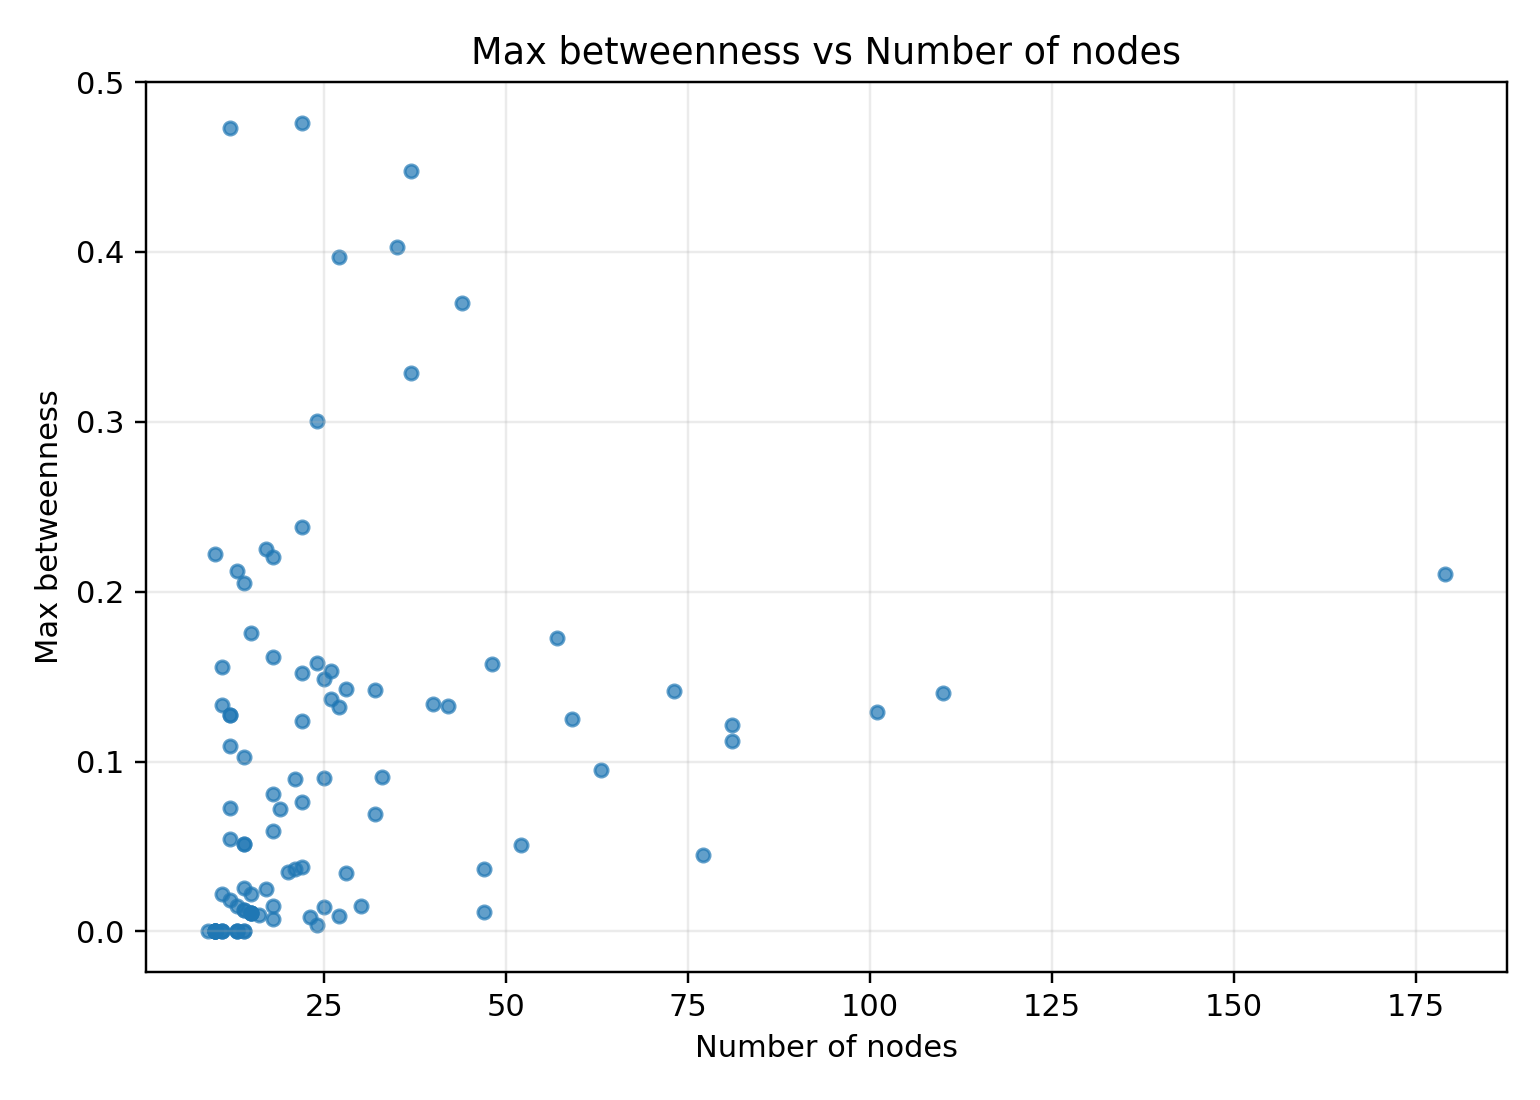
\includegraphics[width=0.45\textwidth]{images/TASK3/metrics_betweenness_max_vs_n_nodes.png}
    \caption{Average (left) and maximum (right) betweenness centrality vs.\ network size.}
    \label{fig:betweenness}
\end{figure}\\
\textbf{Betweenness centrality.}  
As shown in Fig.~\ref{fig:betweenness}, average betweenness remains low and independent of size, indicating that flows are not dominated by specific nodes.  
Maximum betweenness, however, varies considerably: some networks rely on a few bridge nodes, while others distribute flows more evenly.\\
\begin{figure}[h!]
    \centering
    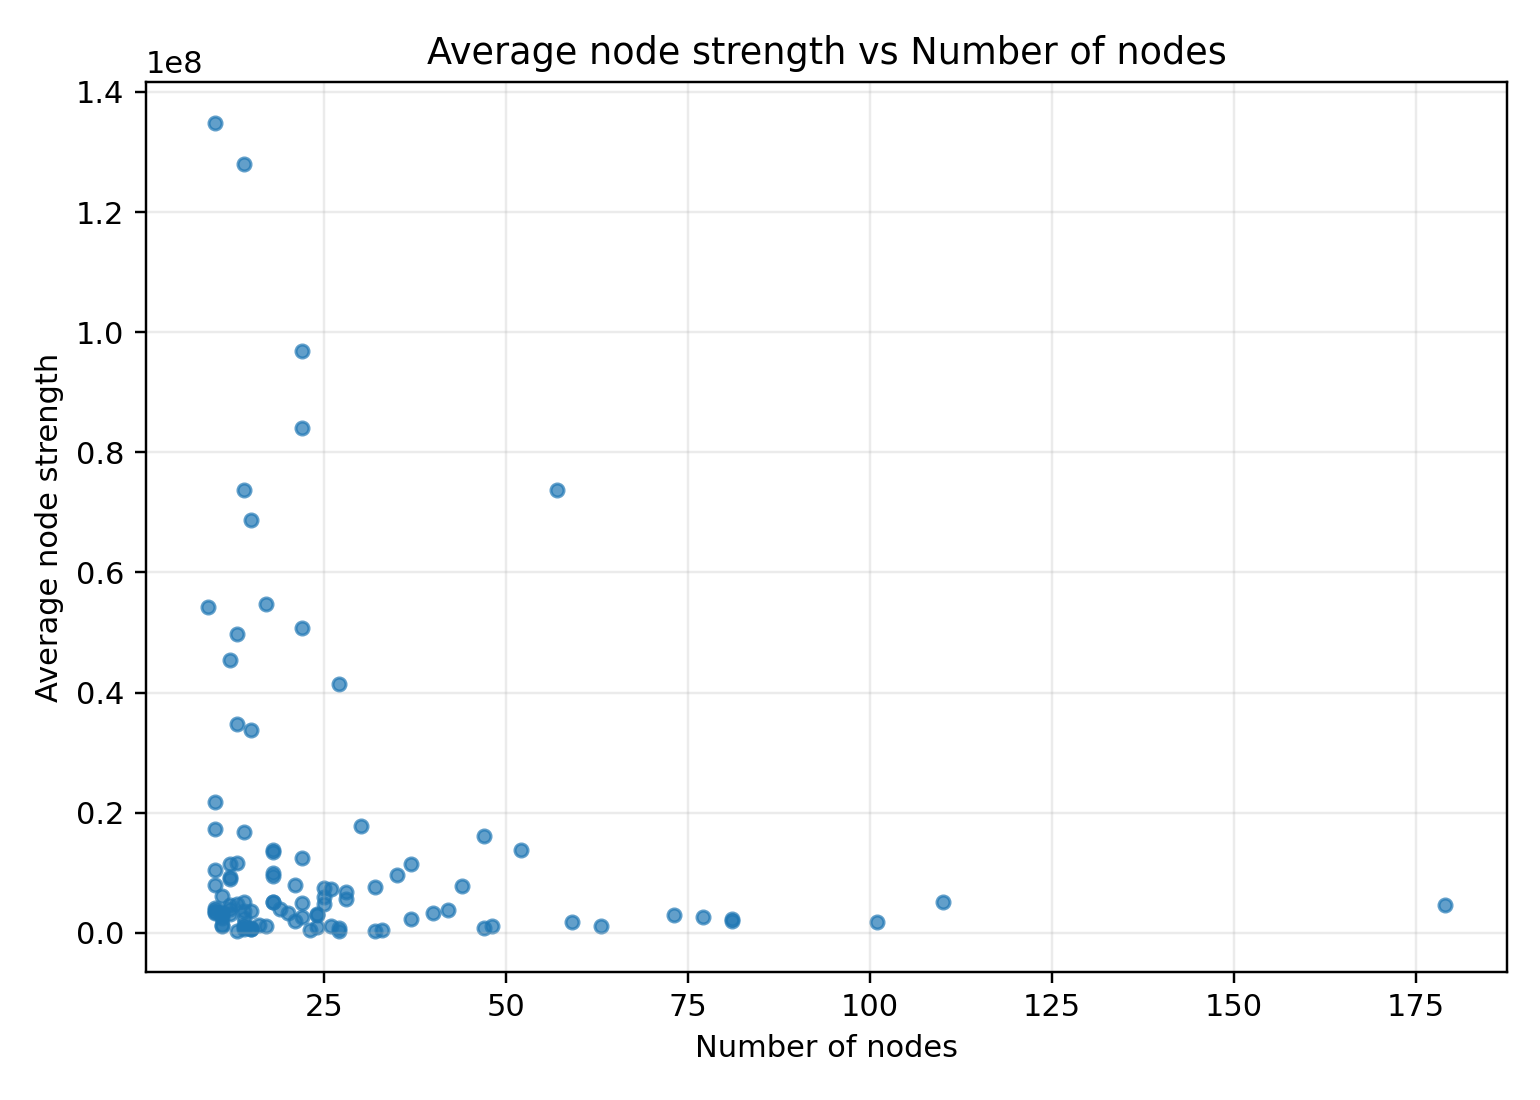
\includegraphics[width=0.45\textwidth]{images/TASK3/metrics_avg_strength_vs_n_nodes.png}
    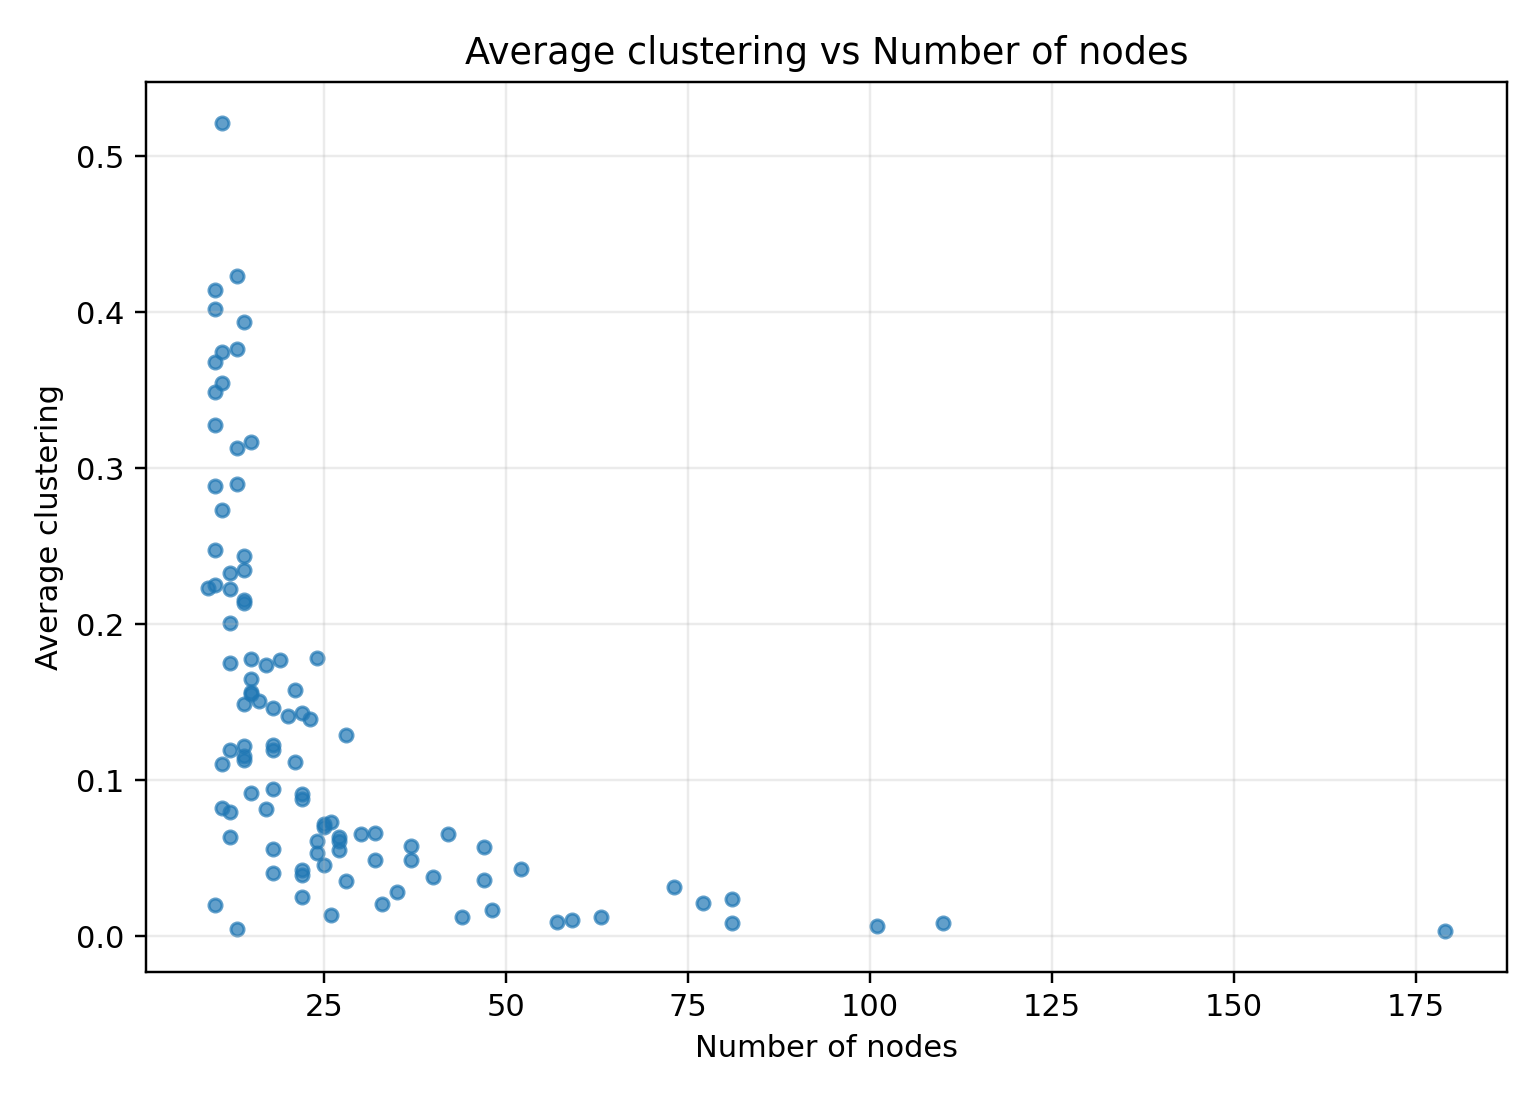
\includegraphics[width=0.45\textwidth]{images/TASK3/metrics_avg_clustering_vs_n_nodes.png}
    \caption{Average node strength (left) and clustering coefficient (right) vs.\ network size.}
    \label{fig:strength_clustering}
\end{figure}\\
\textbf{Strength and clustering.}  
Figure~\ref{fig:strength_clustering} shows that average strength decreases with network size, as weights spread across more nodes.  
Clustering is low and declines as networks grow, indicating weaker local cohesion.  
Together, this suggests that larger SCI subnetworks are more diffuse both globally and locally.\\
\begin{figure}[h!]
    \centering
    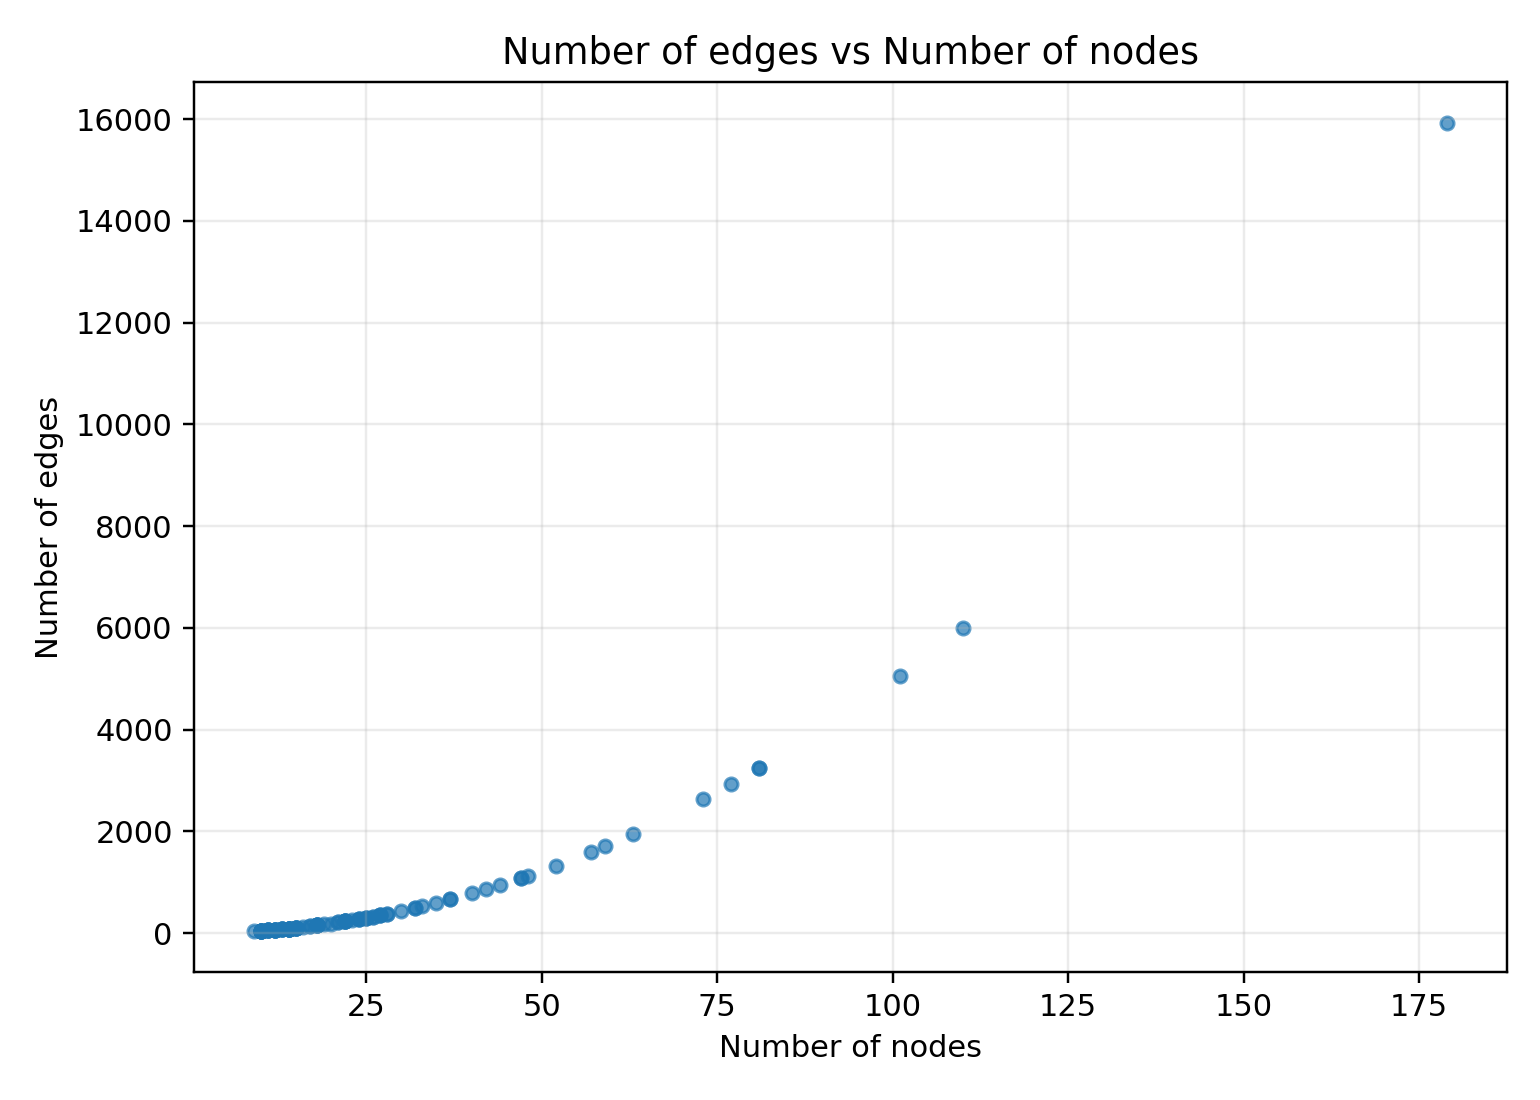
\includegraphics[width=0.45\textwidth]{images/TASK3/metrics_n_edges_vs_n_nodes.png}
    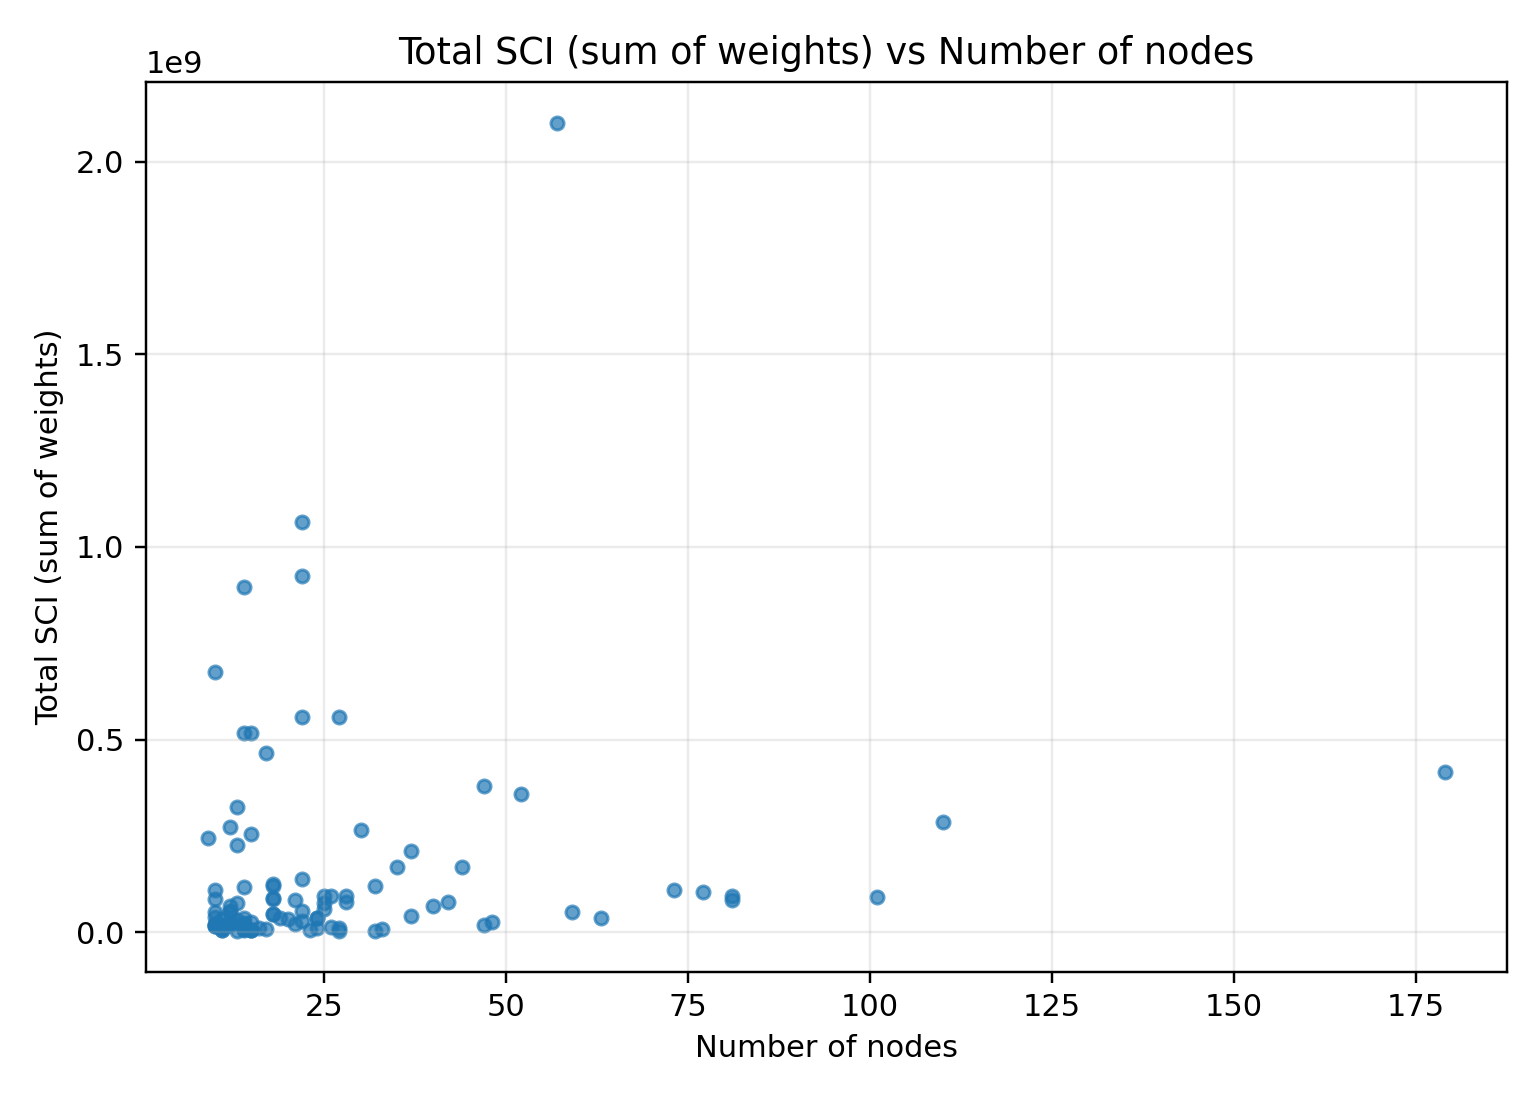
\includegraphics[width=0.45\textwidth]{images/TASK3/total_sci_vs_n_nodes.png}
    \caption{Number of edges (left) and total SCI weight (right) vs.\ network size.}
    \label{fig:edges_weight}
\end{figure}\\
\textbf{Edges and total weight.}  
As seen in Fig.~\ref{fig:edges_weight}, the number of edges grows superlinearly with nodes, confirming the density of SCI graphs.  
Total SCI weight also scales with size but varies widely across countries, reflecting demographic and usage differences.




\newpage